\section{Background}
\subsection{Multi-Layer Perceptron}
\begin{frame}[c]{Multi-Layer Perceptron}
    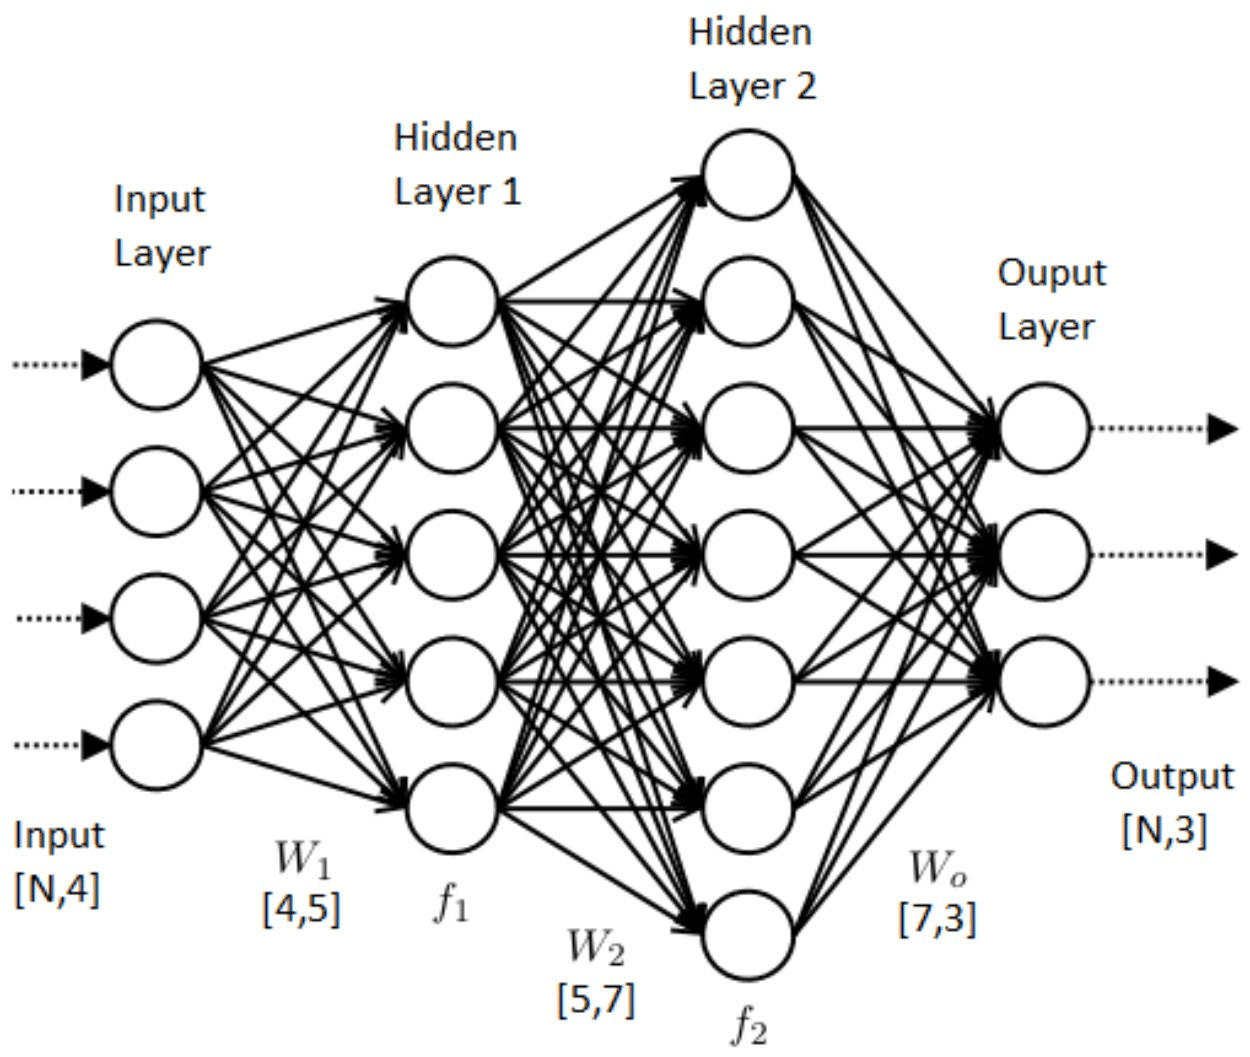
\includegraphics[height=0.85\textheight]{dense_1} \\
    \normalsize
    \gray{Image Source: Public Domain}
    \pnote{
    Classic Dense FF \\
    has some arbitrary nonlinear activation function
    }
\end{frame}

\subsection{Activation Functions}
\begin{frame}[c]{Common Activation Functions}
    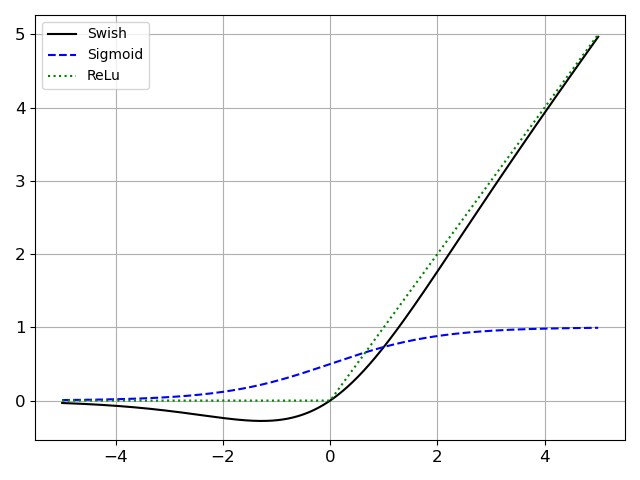
\includegraphics[height=0.75\textheight]{sigmoid_swish_relu} \\
    $swish(x) := x * sigmoid(x)$ \\
    \gray{Image Source: \cite{chen_deep_2021}} \hspace{1cm}
    SwiGLU introduced by \cite{shazeer_glu_2020}
    \pnote{
        GLU = Gated Linear Unit, sigmoid is one too \\
        basically vectorization of activation function
    }
\end{frame}

\subsection{Missing Connections}
\begin{frame}[c]{Dropout I}
    \large
    \textbf{Problem:} neural network training results in highly specialized feature adaptations (overfitting) \\
    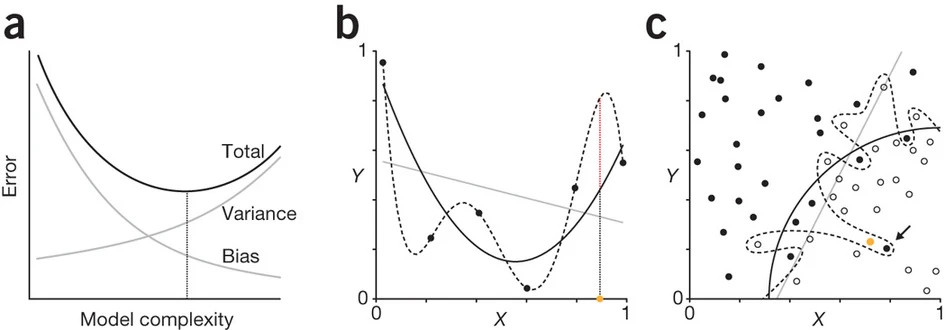
\includegraphics[width=\textwidth]{overfitting} \\
    \normalsize
    \gray{Image Source: \cite{lever_points_2016}}
    % "Complex co-adaptations can be trained to work well on a training set, but on novel test data they are far more likely to fail than multiple simpler co-adaptations that achieve the same thing." \cite{srivastava_dropout_2014}
    \pnote{
        benefits: generalization of features across multiple nodes, \\
        which makes them less pronet to overfitting \\
        \\
        For some reason, not used by a lot of modern LLMs
    }
\end{frame}

\begin{frame}[c]{Dropout II}
    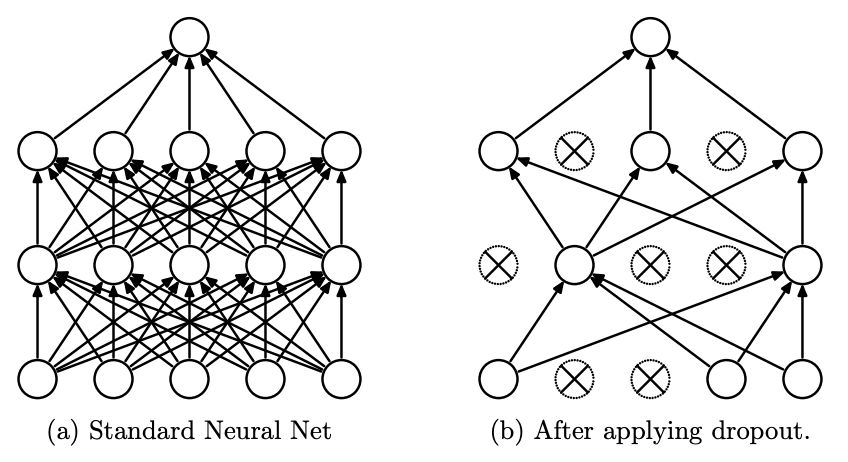
\includegraphics[width=\textwidth]{dropout} \\
    \gray{Image Source: \cite{srivastava_dropout_2014}}
    \pnote{
        Dropout arbitrarily removes neurons during training \\
        => no reliance on individual features \\
        \\
        Effectively results in an ensamble of different \\
        networks, averaging the output during testing. \\
        Powerful method for regularization \\
        \\
        Well-known mechanism for Random Forests
    }
\end{frame}


\subsection{Going Deeper}
\begin{frame}[c]{Residual Connections}
    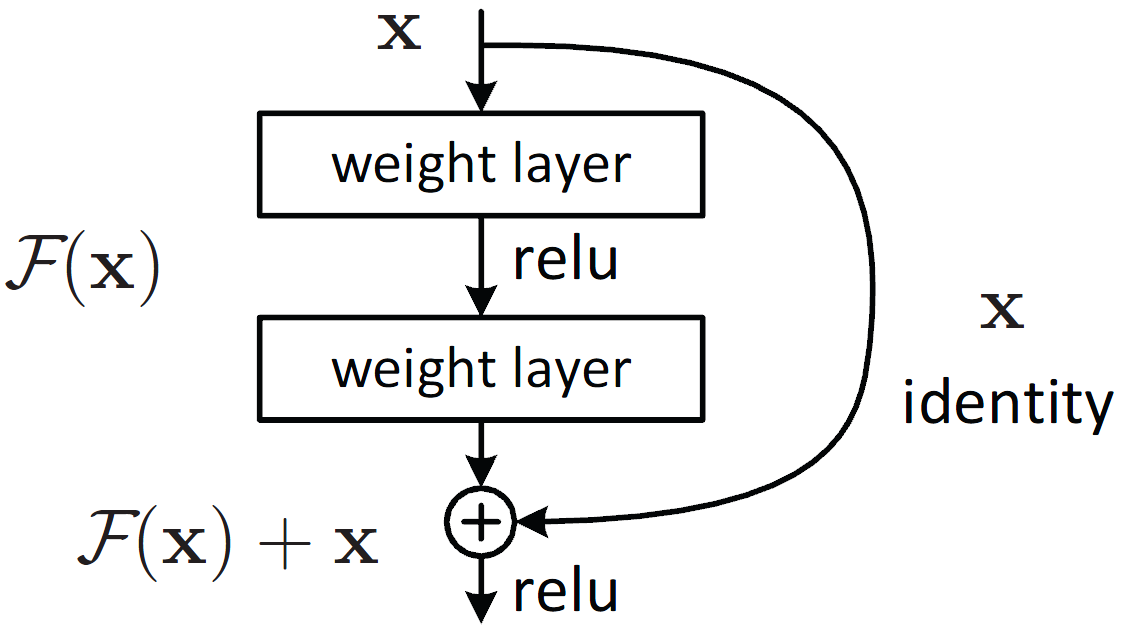
\includegraphics[width=\textwidth]{resnet} \\
    \gray{Image Source: \cite{he_deep_2016}}
    % \large
    % \newline
    % \newline
    % \pause
    % \textbf{Also:} Feature Pyramid Networks \cite{lin_feature_2017} in CV
\end{frame}


\begin{frame}[c]{Perplexity}
    Measure for language modeling capacity
    \todo{build slide}
\end{frame}
